\documentclass[10pt,a4paper]{report}
\usepackage[latin1]{inputenc}
\usepackage{amsmath}
\usepackage{amsfonts}
\usepackage{amssymb}
\usepackage{graphicx}
\author{Michael C. Kunkel}
\newlength{\figwidth}
\setlength{\figwidth}{0.9\columnwidth}

\newlength{\qfigheight}
\setlength{\qfigheight}{0.25\textheight}

\newlength{\hfigheight}
\setlength{\hfigheight}{0.5\textheight}
\begin{document}
	To calculate the track-efficiency systematic uncertainty, the calculation was redone as described in Sec. 6.2 of the analysis note. The track-efficiency for the systematic study had a binning scheme of $\theta$, $\phi$, Fig.~\ref{fig:toteff_protnew}, instead of the $\theta \sin\phi$, $\theta \cos\phi$ binning seen in Fig. 31 in the analysis note.
	
\begin{figure}[h!]\begin{center}
		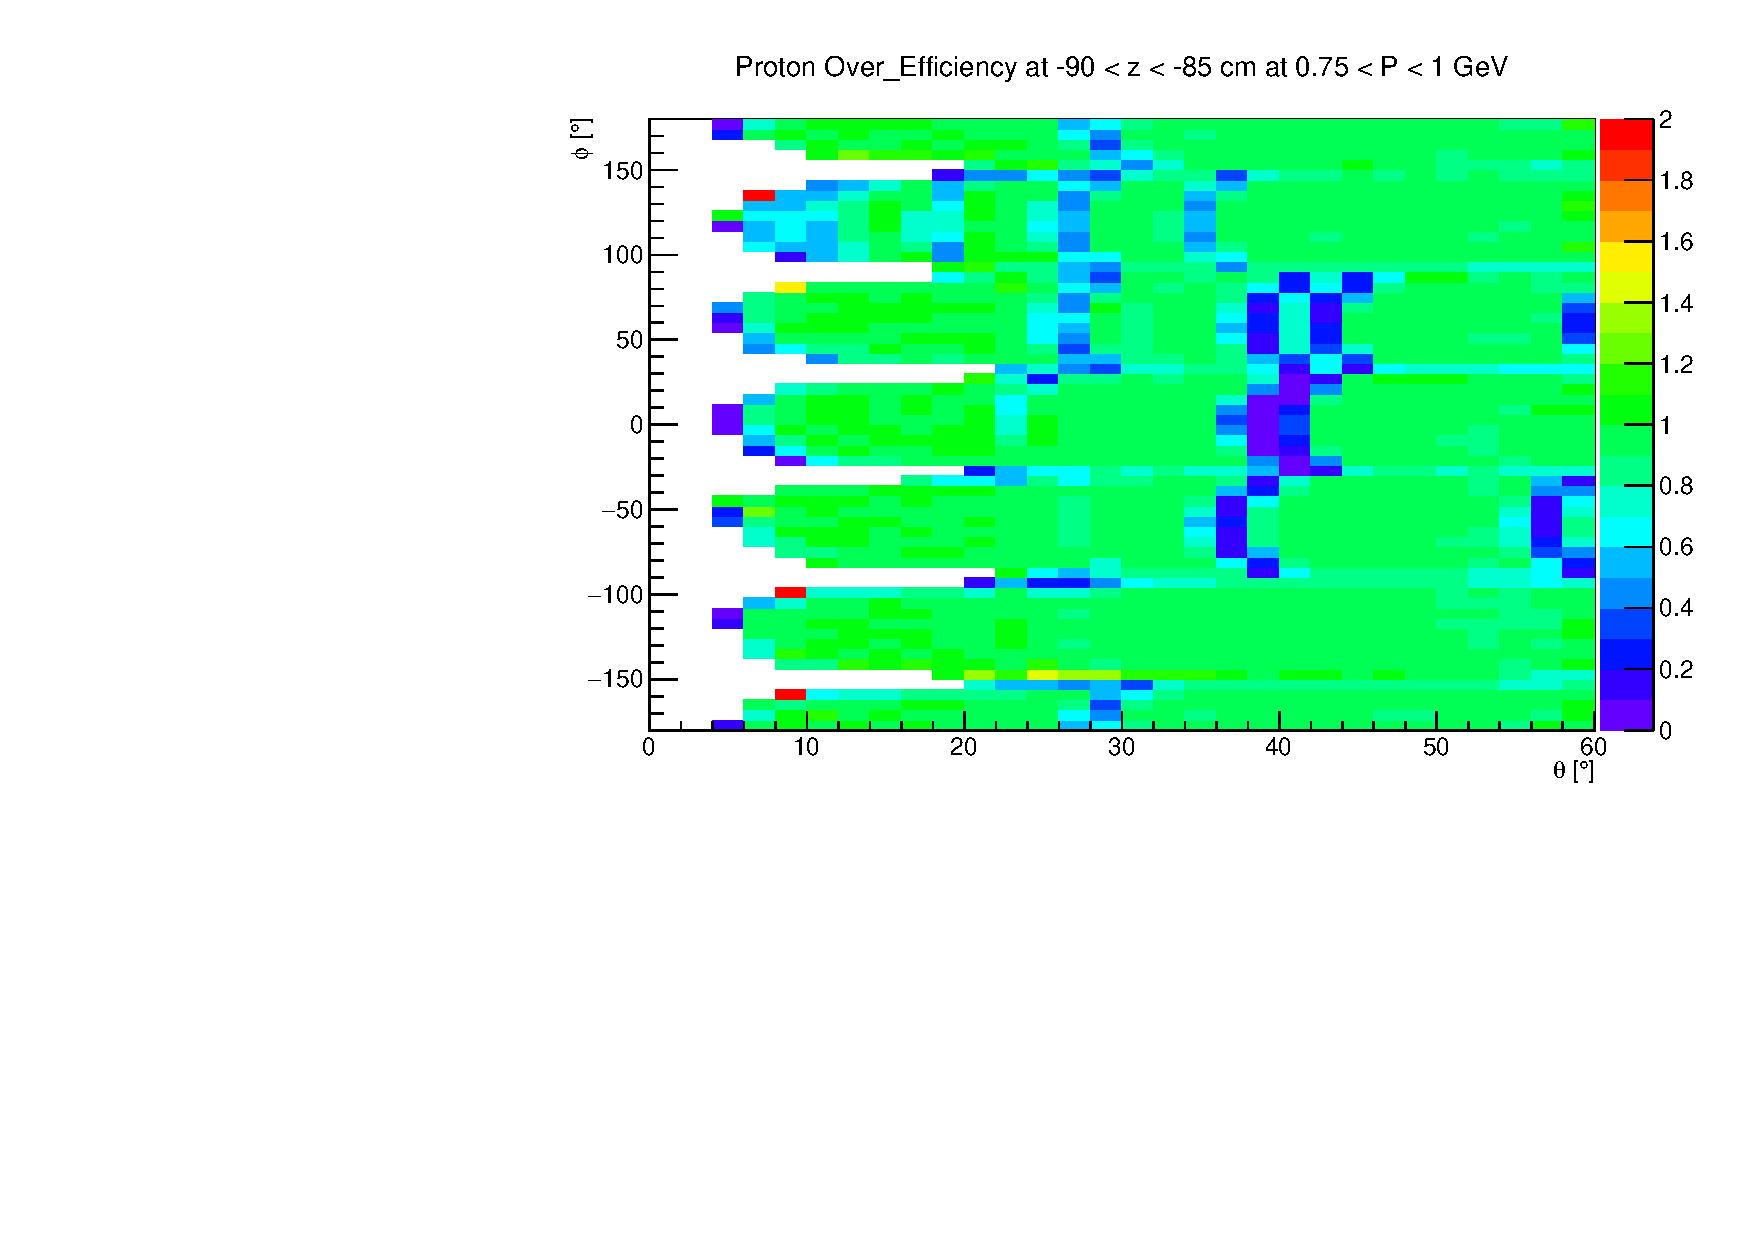
\includegraphics[width=1.1 \figwidth,height=\hfigheight]{/Users/michaelkunkel/WORK/GIT_HUB/Pi0_Papers/ANALYSIS_NOTE/RESULTS/NewEffPlot.pdf}
		\caption[$\phi$ vs. $\theta$ plot showing the over-efficiency of simulating the proton with z-vertex $-90\textless z\textless-85$~cm and momentum $0.75\textless p \textless 1$~GeV from a 2 charged track reaction]{\label{fig:toteff_protnew} $\phi$ vs. $\theta$ plot showing the over-efficiency of simulating the proton with z-vertex $-90\textless z\textless-85$~cm and momentum $0.75\textless p \textless 1$~GeV from a 2 charged track reaction.}
\end{center}\end{figure}
		
Three-charged track-efficiency values from the initial procedure, described in Sec. 6.2, were compared to the values from this new binning. Since both techniques are not known quantities, the method for calculating the error between the is;
\begin{align}
	\Delta = \frac{x_{previous} -x_{new} }{\frac{x_{previous} +x_{new}}{2}}
\end{align}	
where $x_{previous}$ is a value of a three-charged track-efficiency from the mapping of Sec~6.2 and $x_{new}$ is a three-charged track-efficiency from the mapping from the new set of figures derived for this systematic calculation.

Since both values are corrections, it makes little statistical sense to promote one to a "known value", therefore the only appropriate method to measure the error between the values is to use the percent difference method. In this method the denominator is the average value between the two hypotheses, hence the factor of 2.


This accumulative value is shown in Fig.~\ref{fig:toteff_error} fitted to a double-Gaussian distribution function along with a second order polynomial;
\begin{figure}[h!]\begin{center}
		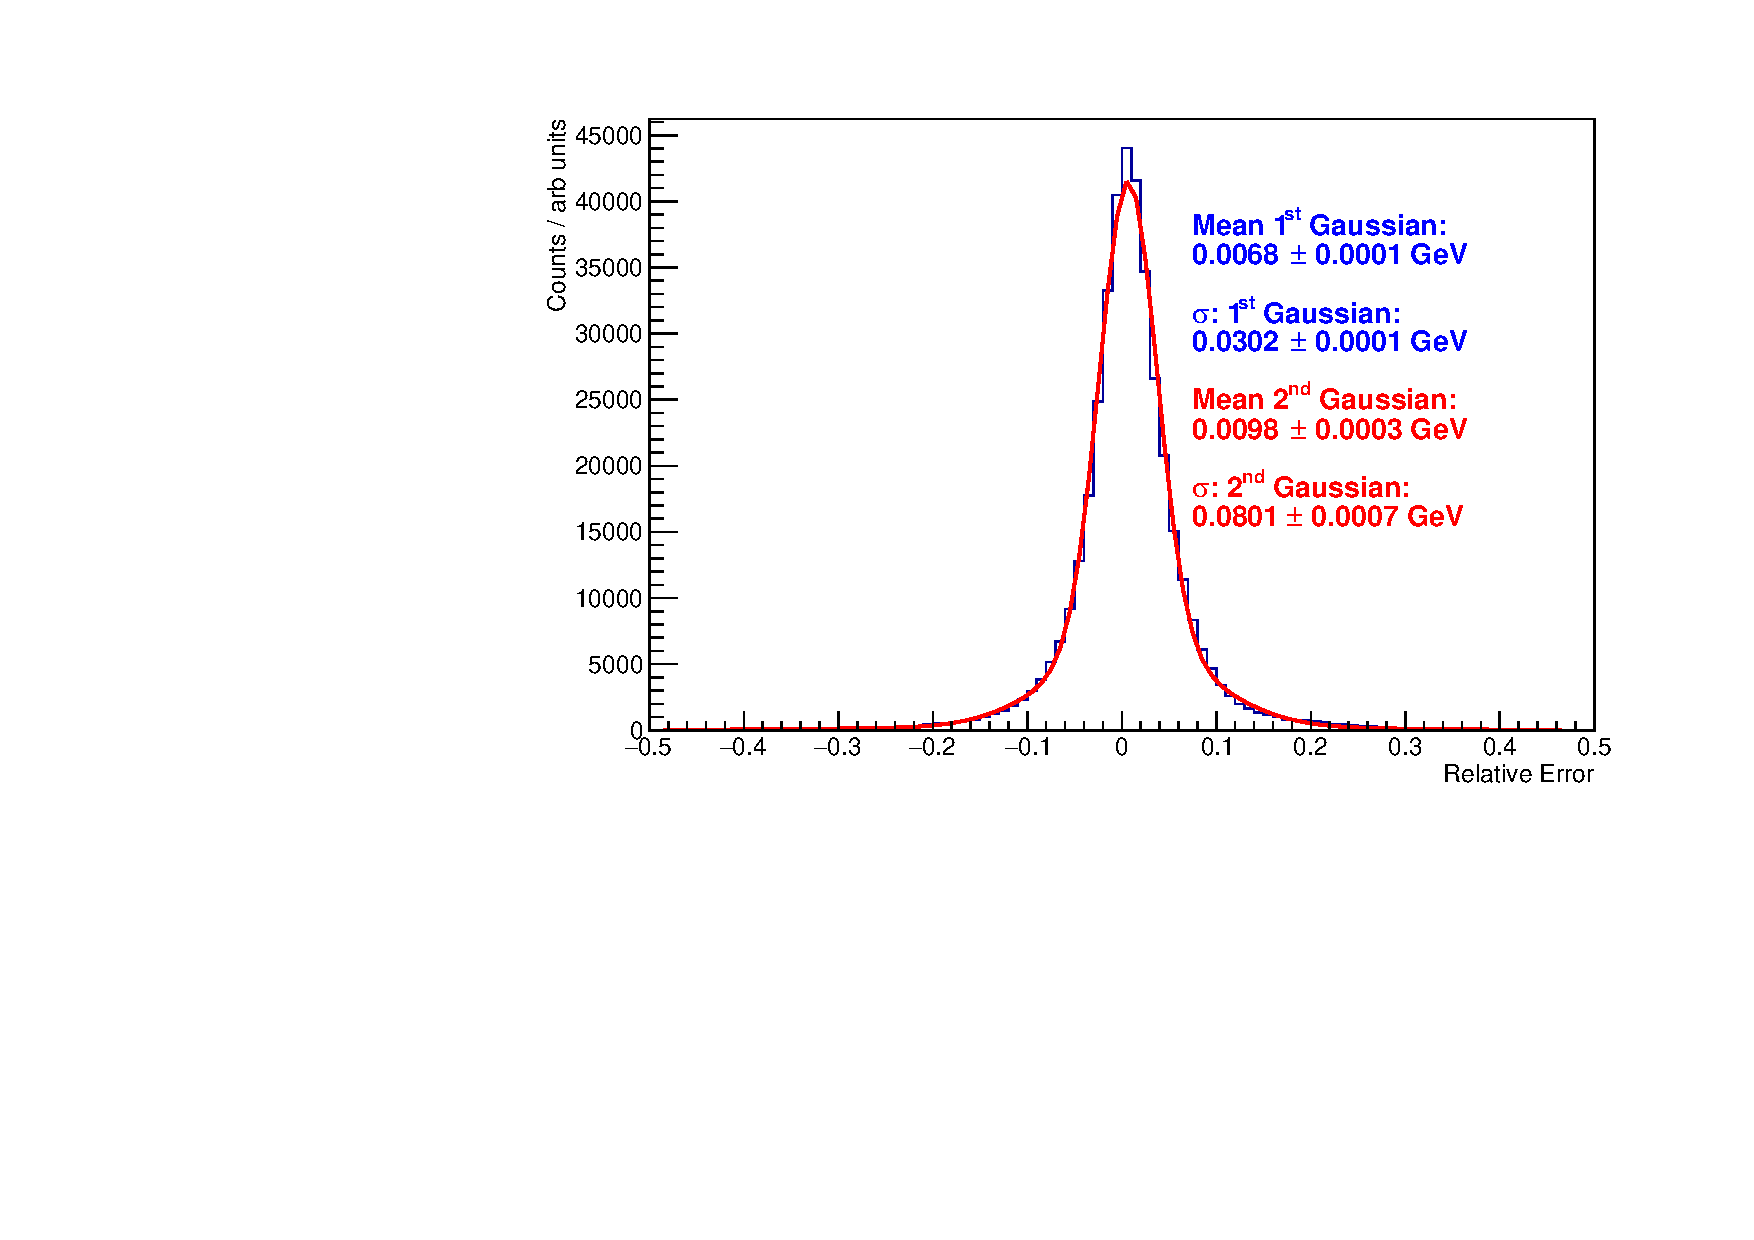
\includegraphics[width=1.1 \figwidth,height=\hfigheight]{/Users/michaelkunkel/WORK/GIT_HUB/Pi0_Papers/ANALYSIS_NOTE/RESULTS/NewEffPlotSys.pdf}
		\caption{Relative error calculated between the two sets of track efficiencies.}\label{fig:toteff_error}
\end{center}\end{figure}
in which the average error between the two methods can be deduced from the largest value of a Gaussian mean, 0.0098 or 0.98\%.		
This value has been changed in the overall systematic uncertainty calculation in the analysis note. The results to be reported are not changed, in systematics, because the difference of the overall systematic are negligible between the previous reported uncertainty and this reported uncertainty. This is shown in Fig.~\ref{fig:toteff_DIFF}.
\begin{figure}[h!]\begin{center}
		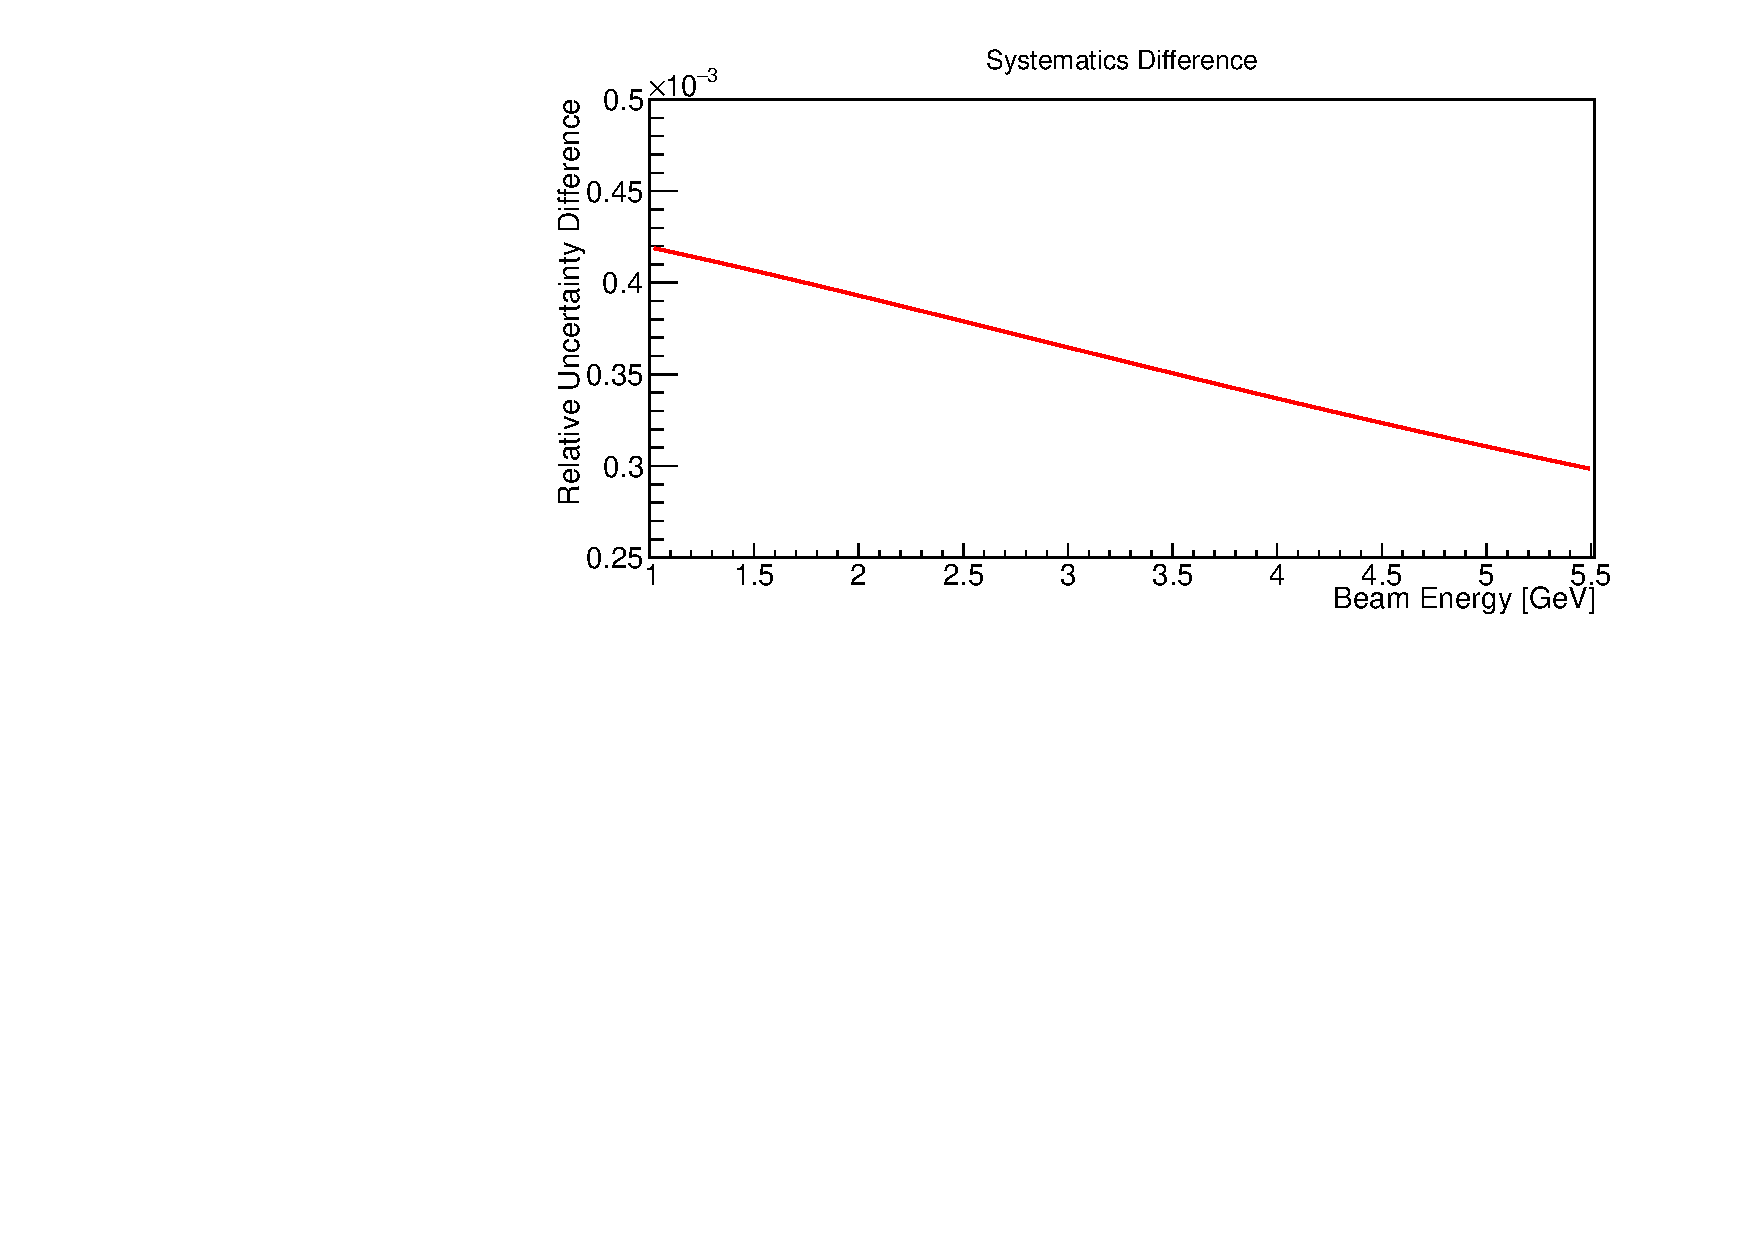
\includegraphics[width=1.0 \figwidth,height=0.9\hfigheight]{/Users/michaelkunkel/WORK/GIT_HUB/Pi0_Papers/ANALYSIS_NOTE/RESULTS/All_SystematicsDiff.pdf}
		\caption{Relative error difference between the two sets of track efficiencies uncertainties reported.}\label{fig:toteff_DIFF}
\end{center}\end{figure}
\end{document}